\documentclass[main.tex]{subfiles}

\begin{document}

\section{Configuration System}
\label{section: configuration}
\textit{this section goes over the general requirements of a configuration system for the pCT project and how it is implemented. It will go over the GUI designed for the configuration and its functionality, along with the API it uses to receive and transmit data. A database solution is presented, using MongoDB to store configuration sets, lastly, a ramp-up algorithm is described and implemented that is to be used in the powering on sequence of the \gls{dtc} \notinmain{ha et underkapittel om mongoDB database og data oppsett: json-format etc.}}



\subsection{Overview}
The microcontroller on the \gls{mb} is responsible for directly monitoring and controlling the power delivery to the 12 strings of its respective layer. It contains registers that allow for modifying PWELL voltage, custom functions accessed by the CTRL registers, and threshold values for each measurement. The microcontroller has eight registers that handle how it will monitor the 12 strings for its respective layer. Seven registers determine the threshold values for DVDD, AVDD, PWELL, and temperature. The last register is the enable signal, which determines how many strings the board will turn on. DVDD, AVDD, and PWELL have two threshold levels, threshold 1 is a warning threshold giving an error message, and threshold 2 is a critical threshold that will automatically turn off all strings if it is exceeded. Temperature only has one threshold value, and the microcontroller will turn off the strings if it is exceeded. The address map of the microcontroller is given in appendix \ref{appendix: register_map}.

Each layer can have different nominal threshold values for voltage and current, and therefore, it is necessary to be able to change these values as we test the strings. A complete set of threshold values for all strings in each layer of the \gls{dtc} will be referred to as a configuration set. The configuration sets must be stored in a database, and MongoDB was chosen for storing the sets; we will discuss the database more in \autoref{ssec: mongo}.

All this leads to a requirement for a user-friendly configuration system that can configure the microcontrollers through IPbus, store configuration sets, and power on the \gls{dtc}. Furthermore, these parts must be developed modular and generic to make the system scalable and easy to modify.

\subsection{Configuration API}
\label{ssec: mcu_api}
IPbus sends and retrieves information between the control software and the MB Hub. IPbus has a software library, uHAL (Hardware Access Library), that provides end-user API for C++ and Python. For this project,  Python is used to interface with uHAL and IPbus. This \gls{api} can issue read and write commands to the IPbus module on the\gls{fpga} and dispatch these commands in a single packet. \autoref{ssec: IPbus} talks more in detail about the IPbus software and how to implement it in Python. uHAL allows us to send and receive data, but this \gls{api} is not sufficient for communicating with the microcontroller; there must be an additional interface that has functions for our specific FPGA design and the \gls{pcs} as a whole. Following the principles of \gls{oop}, it is natural to encapsulate the properties of the API into two interfaces, one for the MB Hub and one for the microcontroller on the \gls{mb}.

\subsubsection{IPbus API}
The IPbus \gls{api} contains functions for read and write commands using uHAL, broadcast functionality using the global module, and enabling/disabling the com modules for individual layers. This interface Python class is named "ipbus low interface".

An important part of the \gls{api} is the "issue" functions. \autoref{ssec: IPbus} discusses how IPbus benefits from packing data in larger payloads before dispatching them, and that is the purpose of the "issue" functions. The "issue" functions loads the data request in a payload without sending it to the MB Hub. This can be used to optimize the communication chain between the control software and the microcontroller, by limiting the amount of network dispatches performed.

\subsubsection{Microcontroller API}

The \gls{api} for the microcontroller must interface with the microcontroller, and by extension, the MB Hub. Therefore, the microcontroller \gls{api} uses the IPbus \gls{api} as a lower level communication interface. The microcontroller \gls{api} has similar functions as the IPbus \gls{api}, except it uses namedtuples to create the data header for communicating with the microcontroller.

Namedtuples is a container in Python with user defined parameters. The address map of the microcontroller has been defined in a separate package using namedtuples, and the \gls{api} uses these namedtuples for retrieving information about address value, measurement type, and so on. This serves two purposes





The \gls{api} for the microcontroller must interface with the microcontroller, and by extension, the IPbus module. Therefore it is built on top of the IPbus \gls{api}, i.e. the microcontroller class instantiates an IPbus \gls{api} object inside its constructor. This higher level \gls{api} have functions that formats the data header depending on address and data, and then sends it to the appropriate module on the \gls{fpga}. An important detail of the \gls{api}s is the difference between the get/set functions and the issue read/issue write functions. The difference is the use of the dispatch-command from the uHAL library. The get/set functions performs a dispatch of its request immediately, while the issue read/issue write functions only issues a read/write request with no dispatch after. The purpose of the issue functions is to be able to issue many IPbus commands at once, and then dispatch them all in one large packet. The system would be significantly slowed down if it had to dispatch every command one-by-one, and the issue-functions is more flexible for parallel configuration of the layers. By sending many commands at once, we let the \gls{fpga} handle the configuration data of every layer in parallel, which fully utilizes the \gls{fpga} architecture. Aditionally, the IPbus protocol is most efficient when sending large packets of data at once, making the issue-functions even more time efficient than the get/set functions.

The main challenge of using issue functions is handling the handshake values from the RX register in the com module. The RX register is connected to a \gls{fifo}, and this \gls{fifo} is filled with a handshake value for each write request performed and a read requests inserts the read value from the microcontroller to the same RX-register. Using the issue command to perform many requests at once means that you need to keep track of the number of requests and what the expected handshake value should be for each write request. This process will require high level functions to manage the \gls{fifo} and handshake values while performing a large amount of requests, notably when configuring the \gls{dtc}. Furthermore, the configuration system will need a ramp-up-algorithm for powering on the strings in each layer, this algorithm will be discussed in section (powering algorithm).

From this, it is natural to create another layer of abstraction that we can use to interface with in the configuration system. This interface will contain functions specific for configuring the \gls{dtc} and will be called "config api". The hierarchy for the abstraction of interfaces is given in \autoref{fig: interface_hierarchy}.



\begin{figure}[!ht]
    \centering
    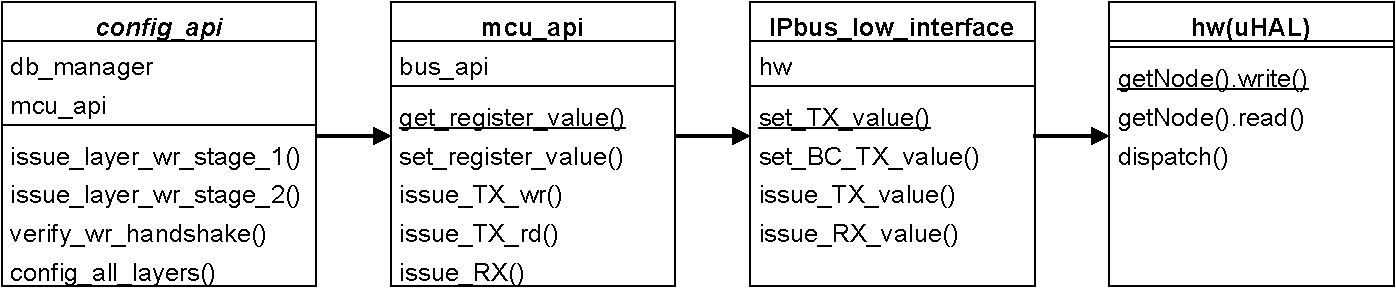
\includegraphics[width=17cm, scale=4]{images/interface_hierarchy.pdf}
    \caption{Interface hierarchy for the configuration system.}
    \label{fig: interface_hierarchy}
\end{figure}
\FloatBarrier

Setting up the configuration system only requires the user to instantiate a \textit{config api} object in a python script. This class \gls{api} has several functions for handling data retrieved from the database and perform operations in the configuration process, like verifying handshakes and ramp-up algorithm. \textit{config api} has two functions for issuing configuration commands down to the \gls{dtc}, stage 1 and stage 2. These two will be discussed more in \autoref{ssec: power_algo}. Most of the functions of the \textit{config api} is different parts of the powering-on algorithm and the \textit{config all layers}-function starts up the configuration process using the other functions, along with gradually turning on each string one-by-one. The \gls{api} also has functionality for debugging the power usage of the strings. As mentioned in section blablabla (microcontroller in MB subsection), the microcontroller contains an enable scan function, for testing the current consumption of each string. The \textit{verify string currents} function in the \gls{api} starts the enable scan and then retrieves the current values from the microcontroller. This allows us to detect strings with unusually high current consumption.



\subsection{Powering algorithm}
\label{ssec: power_algo}
Powering on and configuring the strings of the \gls{dtc} comes with its own challenges. Tasks such as enabling layers, sending configuration data and verifying handshakes must be performed every time the system is turned on. The calorimeter is made of 43*12 strings that all consume a significant amount of current. There are several constraints that must be considered while powering on such a system. Powering on all strings at once would cause a power spike that could damage equipment if not handled correctly. A solution to this is to develop a ramp-up algorithm that turns on each string one by one, gradually increasing the power level of the strings. 

The algorithm must perform these tasks:

\begin{itemize}
    \item Get the configuration values from the database.
    \item send write requests to every layer.
    \item verify handshake values from the write requests.
    \item Turn on each string sequentially and verify they do not get turned off by the microcontroller.
\end{itemize}

The configuration \gls{api} contains functions that perform handshakes and stages write commands to IPbus, and the \textit{config all layers}-function wraps these together to perform the configuration. The stage 1 and stage 2 functions is responsible for retrieving the values from the database and issuing the write requests for the specified layer. Stage 1 issues the write requests for the registers in the database made of only a single value, stage 2 handles the enable signal and the threshold values made of a dictionary.

The reasoning behind having two stages is twofold, to prevent unnecessary write operations and to ensure more readable, concise code. Only 4 of the 8 registers needs to be changed when a new string is turned on, the three threshold values for AVDD, DVDD and PWELL, as well as the enable signal, which turns on the next string. If a single function issued all the write-requests, then we would have to configure twice as much registers each time a string turned on. Stage 1 issues the write requests for the 4 registers that is static during the ramp-up process, while stage 2 issues requests to the 4 registers that changes for each string.

The algorithm will first use stage 1 to configure all layers, then use the stage 2 function in a loop, to gradually turn on the strings and set appropriate threshold levels. A flowchart of this procedure is given in \autoref{fig: flow_chart}.

\begin{figure}[!ht]
    \centering
    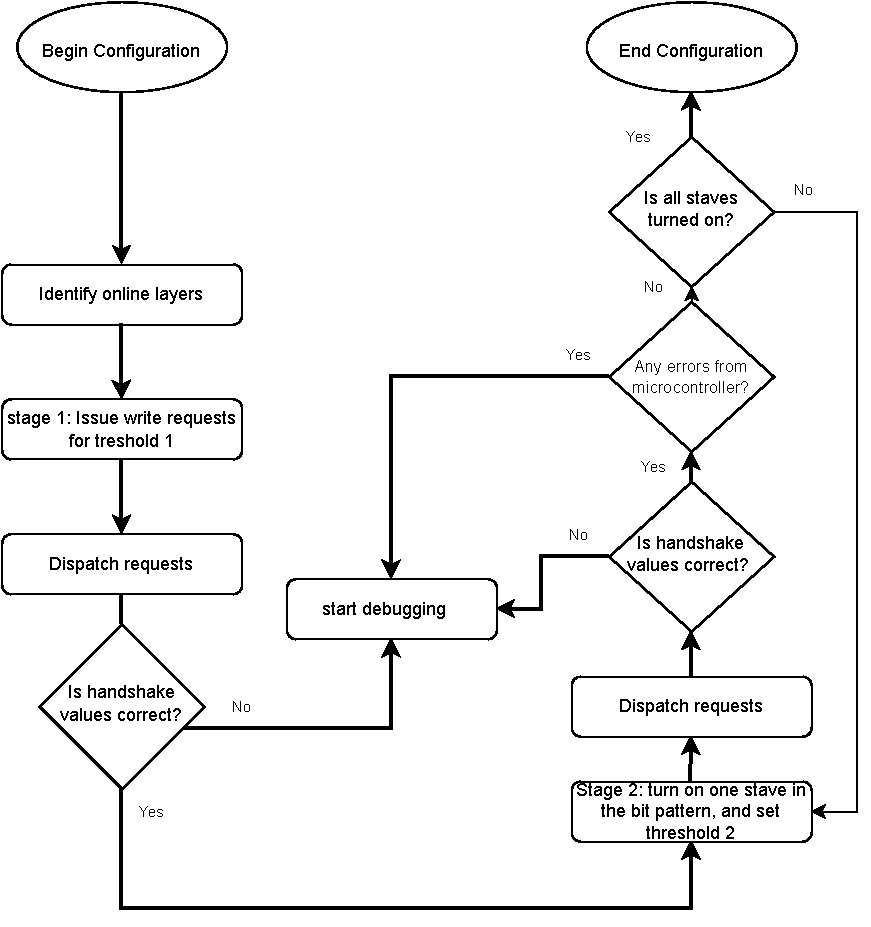
\includegraphics[width=12cm, scale=1.5]{images/new_config_chart.pdf}
    \caption{Flowchart of the configuration function of a single layer.}
    \label{fig: flow_chart}
\end{figure}
\FloatBarrier

The left side of \autoref{fig: flow_chart} shows the flowchart of stage 1, where the warning threshold levels is set, along with temperature limit. Notice it is issuing all the commands first, then dispatches them and verifies handshake values afterwards. "Start debugging" means a error message is given and the program will stop. The right side of \autoref{fig: flow_chart} shows stage 2, where it turns on the strings one-by-one. The \textit{error count} register from the microcontroller is checked at the end of the loop to assert whether any strings were turned off due to high currents.

Turning on the strings one-by-one is a process that depends on the number of strings in use. If 4 of the 12 strings are not in use, then only 8 stages of ramp-up is required for the configuration. There are two options for implementing the loop for all layers, configure for each bit in the enable bit pattern, or only configure the the 1's in the enable bit pattern. \autoref{fig: string_config_timing} shows the two different algorithms for three arbitrary bit patterns.

\begin{figure}[!ht]
    \centering
    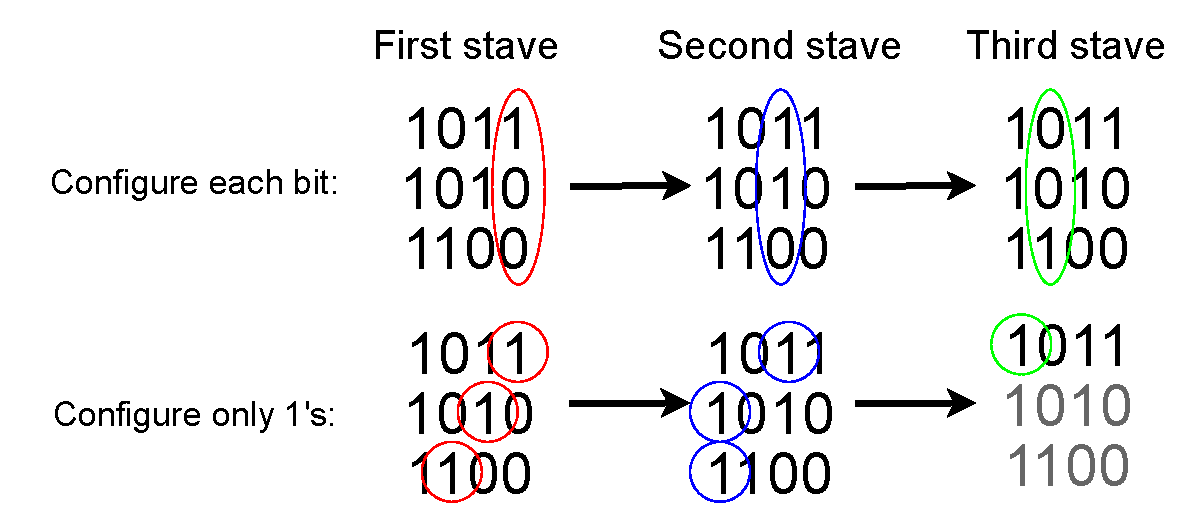
\includegraphics[width=13cm, scale=1.5]{images/string_config_timing.pdf}
    \caption{Example of the two loop algorithms on three arbitrary bit patterns.}
    \label{fig: string_config_timing}
\end{figure}

As seen from the figure, configuring each bit is a slower process. It issues write requests to a layer, even if the next string is turned off in the enable bit pattern, which means it writes redundant data to the microcontroller. The benefit of this type of loop is that it is simple, requiring only a single 12 length loop and it is easy to implement.  Configuring only the 1's is a "smarter" algorithm that skips the 0's in the bit pattern, only issuing write requests for strings that are turned on. As seen in \autoref{fig: string_config_timing}, it will always be as fast, if not faster than configuring each bit. The downside to this algorithm is its complexity, each layer will have a variable amount of loops for its configuration that must be tracked for all 43 layers. This complexity will also lead to the code being more difficult to read.

It was decided to implement the "configure each bit" algorithm in the configuration process, due to it being more modular, resulting in easier to read code that can be modified if necessary. Additionally, we assume in this project that we will always have 12 operational strings for each layer, meaning the "configure only 1's" algorithm is redundant. The "configure only 1's" concept might be worth revisiting in the future if the configuration speed becomes an issue. This is of course only relevant when troubleshooting a few amount of strings, if a whole set of strings is present then "configure only 1's" will not speed up the configuration process.

\subsection{Mongo Database}
\label{ssec: mongo}
As previously mentioned, the database chosen for the configuration is MongoDB. The reason it was chosen is due to it being a popular, open source, noSQL database, with Python API libraries. MongoDB is capable of storing large amounts of data, which is useful for storing many large configuration sets. The APIs will access the database through use of PyMongo library, containing functions for reading, writing and searching the database. The configuration of the readout-chips also implements MongoDB, and using the same database for both systems reduces the modular complexity of the configuration systems as a whole.

The hierarchy of a MongoDB database is shown in \autoref{fig: mongo_chart}.

\begin{figure}[!ht]
    \centering
    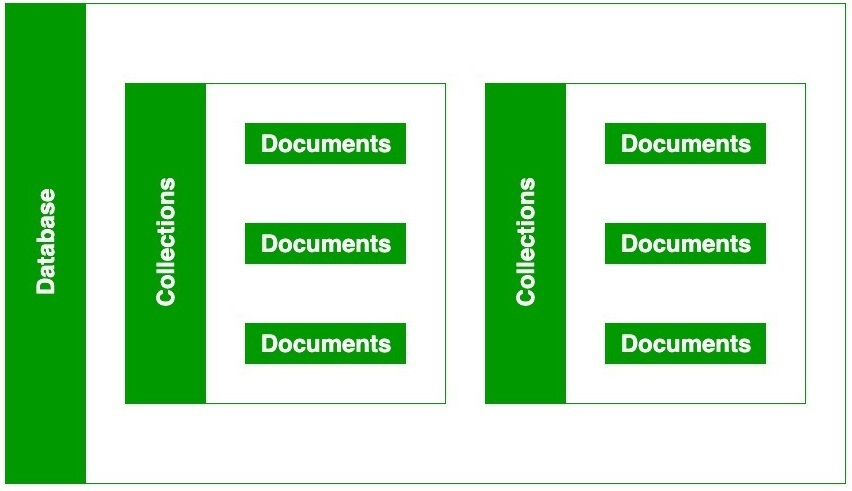
\includegraphics[width=12cm, scale=1.5]{images/mongodb-nosql-working.jpg}
    \caption{Hierarchy of a database in MongoDB.}
    \label{fig: mongo_chart}
\end{figure}
\FloatBarrier

Each database contains user defined collections that each store its own documents. In this project, there is two collections, "Configuration sets", and "Log messages". The former is for storing the different configuration sets and the latter stores the log messages from the \gls{gui}, as is discussed in \autoref{ssec: cgui}.

MongoDB uses JSON as the template for its databases, JSON being a widely used text-based data format for storing and transferring data. A typical example of a MongoDB JSON document is shown below in \autoref{fig: mongo_example}.

\begin{figure}[!ht]
    \centering
    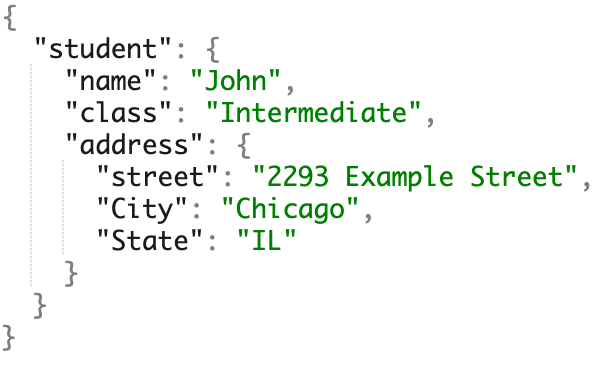
\includegraphics[width=9cm, scale=1.5]{images/mongodb_document_example.png}
    \caption{Hierarchy of a database in MongoDB.}
    \label{fig: mongo_example}
\end{figure}
\FloatBarrier

A document contains fields, and each field contains a corresponding value. This value can be a number, string or a dictionary of sub fields, the address field in \autoref{fig: mongo_example} contains three fields with their own values.
For our purpose, the format of the initial configuration set were not too complex, each field only need to contain a single value and they must be set values for each layer. Additionally, each configuration set must contain a "last updated" timestamp for the sake of documentation, and it must have a field for enabling the com-modules on the \gls{fpga}. Two iterations of the database format were made, the first iteration of this data format is shown in \autoref{fig: json_v1}

\begin{figure}[!ht]
    \centering
    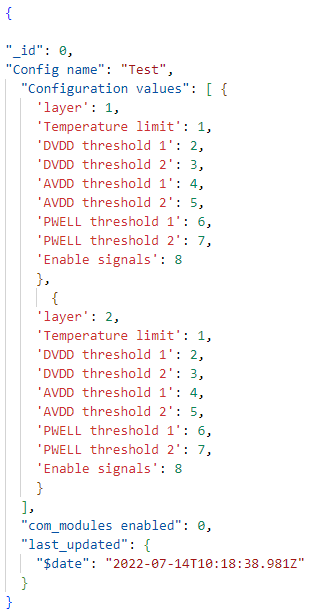
\includegraphics[width=5cm, scale=1]{images/JSON_example_v1.png}
    \caption{First iteration of JSON format of a configuration set.}
    \label{fig: json_v1}
\end{figure}
\FloatBarrier

Each set has a unique name and the configuration values are stored in dictionaries inside the "configuration values" field. The "configuration values" field contains a separate dictionary of each layer, containing the eight threshold values. Retrieving the information using Python is as simple as using a get command for the threshold values.

One of the challenges behind the ramp-up algorithm is that strings' current consumption can wildly vary depending on the quality of the chips on the string. Some strings can use double the current consumption than others and implementing this into the ramp-up process would be next to impossible without having the information on the string's threshold levels. Therefore, the second iteration of the database contains individual threshold values for each stave to alleviate this problem. \autoref{fig: json_v2} shows an outline of this implementation of the database.

\begin{figure}[!ht]
    \centering
    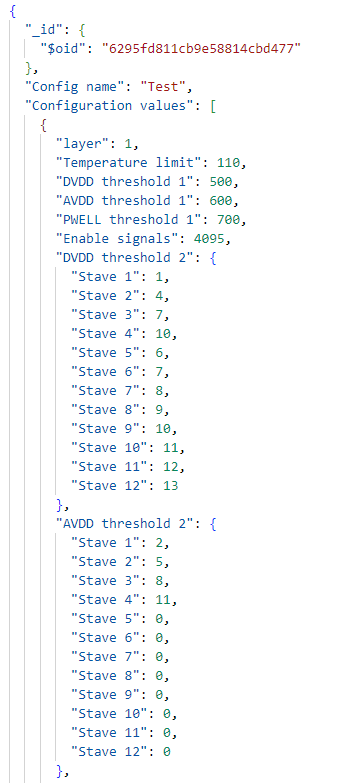
\includegraphics[width=5cm, scale=1]{images/JSON_example_v2.png}
    \caption{Second iteration of JSON format of a configuration set, with for individual strings.}
    \label{fig: json_v2}
\end{figure}
\FloatBarrier

This new iteration is similar to the first, but all the threshold 2 levels for PWELL, DVDD and AVDD is made of a dictionary of values for each string. It is not shown in \autoref{fig: json_v2}, but this format also has fields for last updated and COM modules enabled. The configuration API must sum these string values while performing the ramp-up process, leading to more logic on the software side, specifically for the configuration \gls{api}.

Setting up the database format, and creating new sets is performed with a custom class named \textit{db\_manager}. This class contains functions for communicating with the Mongo database, creating new configuration sets and updating these sets with new values. All formatting of the data happens in this class, the Mongo database does not perform any special functions in regards to manipulating the stored data.



\subsection{Configuration GUI}  
\label{ssec: cgui}
The configuration API contains many functions for setting up the configuration process and managing the Mongo database, but this class requires an end-user interface that not only allows for easily setting up configuration data, but is also user-friendly. A person with no knowledge of the underlying process behind the configuration must be able to load a configuration set from the database and start the configuration of the strings. A logical answer to this problem is to implement a \gls{gui} for the configuration system, but unlike the monitoring system, no specific \gls{gui} exists that is applicable to the configuration, and thus a custom-made \gls{gui} must be implemented.

The basic features the \gls{gui} requires is the ability to load configuration sets from the database and start the configuration with the push of a button. Additionally, the \gls{gui} must also have an "advanced"-tab that allows the user to directly create new configuration sets and insert them into the database, as well as being able to directly modify already existing sets.

Building the \gls{gui} and designing it is performed using Qt Designer, and its Python library, PyQt5 is used to interface the \gls{gui} with our configuration \gls{api} and database. This tool was used to design the \gls{gui} because it is easy to work with and this tool has been used previously to create GUIs for the readout electronics, and this allows us to reuse code.

The class chart for the configuration GUI is given in \autoref{fig: gui_chart}.

\begin{figure}[!ht]
    \centering
    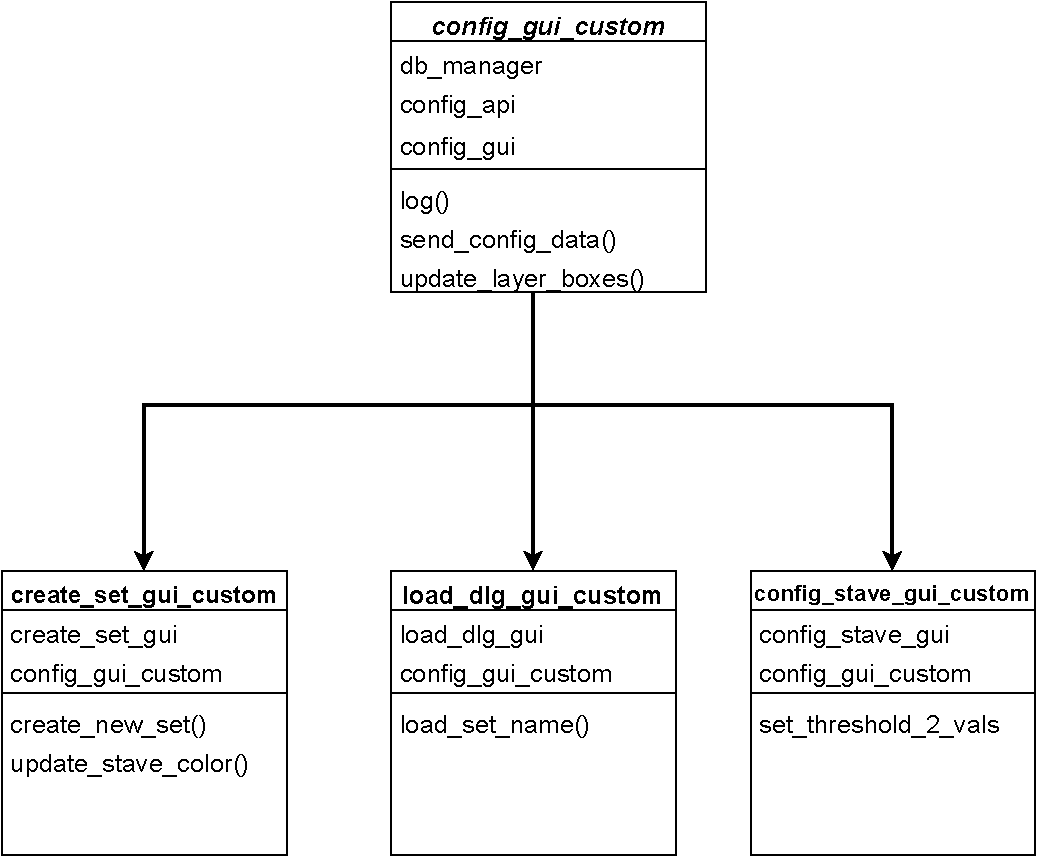
\includegraphics[width=12cm, scale=1.5]{images/gui_class_diagram.pdf}
    \caption{Class diagram of the configuration GUI.}
    \label{fig: gui_chart}
\end{figure}
\FloatBarrier

The GUI is made out of 4 custom python classes, the main class, \textit{config\_gui\_custom} is the main window the user will interact with. The other classes are the windows for creating new configuration sets, loading sets from the database, and setting the individual string threshold values. \textit{config\_gui\_custom} instantiates the configuration \gls{api} and database manager and connects their functions to the GUI buttons.

The main window of the GUI is shown in \autoref{fig: gui_window}, displaying the "basic" tab.

\begin{figure}[!ht]
    \centering
    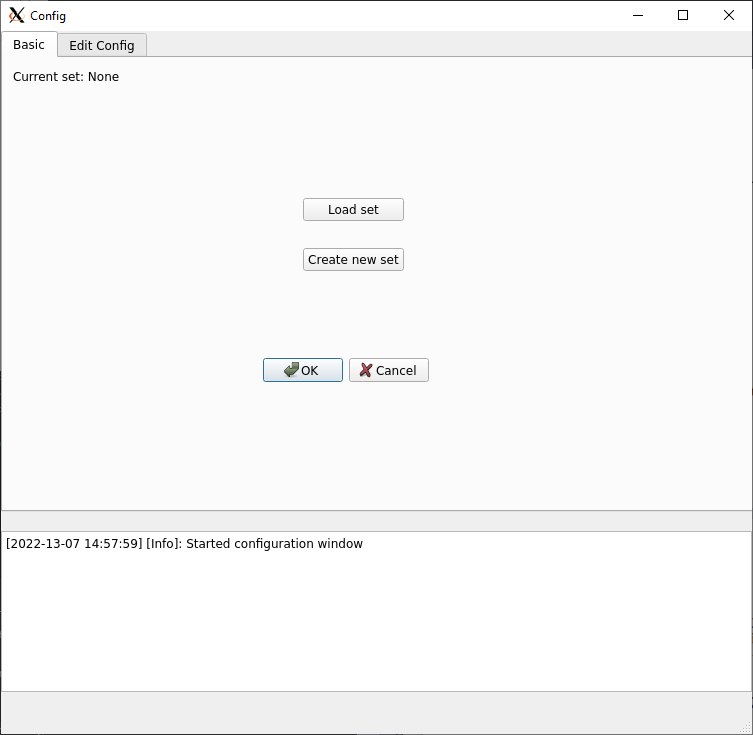
\includegraphics[width=10cm, scale=1.5]{images/gui_main.png}
    \caption{Image of the main window of the configuration GUI.}
    \label{fig: gui_window}
\end{figure}
\FloatBarrier

The window has buttons for loading a set from the database, creating a new set and inserting it into the database, and a confirm or cancel dialog buttons. Upper left of the window shows which configuration set is currently loaded. The window has a log window that informs the user of actions performed, errors, and confirmation messages. These log messages are timestamped and stored in a different collection in MongoDB, giving us more control of the configuration process a typical use case for the "basic" tab is loading set from the database, and then clicking OK, then clicking the "start configuration" button on the main hub GUI to start the configuration process.

Clicking the "Load set" button will open up the a dialog window, showing every set in the database.

\begin{figure}[!ht]
    \centering
    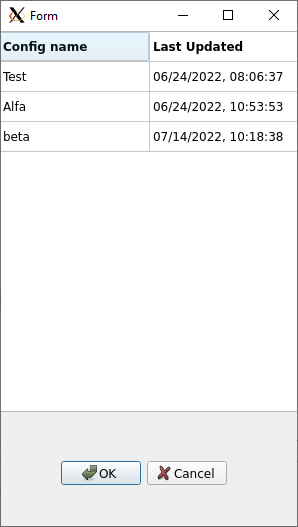
\includegraphics[width=4cm, scale=1]{images/load_dlg_window.png}
    \caption{Image of load set window.}
    \label{fig: load_window}
\end{figure}
\FloatBarrier

As shown in \autoref{fig: load_window}, the window shows every set along with a timestamp of when it was last updated. Choosing a set to load is done by clicking on the row of a set, and then pressing the "OK" button.

The "Edit Config" tab allows for both reading and modifying the threshold values for each set. It is shown in \autoref{fig: edit_tab_window}.

\begin{figure}[!ht]
    \centering
    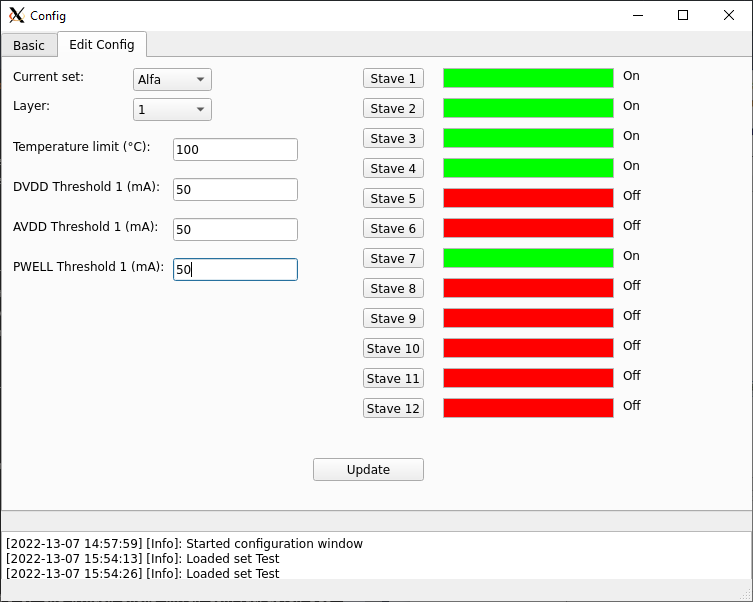
\includegraphics[width=13cm, scale=1.5]{images/config_tab_gui.png}
    \caption{Image of the "Edit Config" tab.}
    \label{fig: edit_tab_window}
\end{figure}
\FloatBarrier

The threshold values can be set for each layer, as well as turning off and on the strings interactively by clicking on its corresponding colored box. The log window will alert the user when any changes are made to a configuration set. This tab is useful for making small changes to already existing sets, but requires the user to be knowledgeable about the structure of the configuration sets to edit them.

The "Create set" button opens up a window identical to the "Edit Config" tab, allowing the user to create a new set. It is not possible to set different values for each layer while creating it, instead, the "Edit Config" tab can be used for that purpose after the set has been created.


\subsection{Configuration Timing}
\label{ssec: con_timing}

Configuring the layers of the \gls{dtc} requires sending multiple write requests through the \gls{pcs} and this process can potentially take a significant time to perform. Debugging the hardware becomes tedious and unrealistic to perform if the the configuration takes several minutes, it is therefore important to ensure the configuration is as fast as possible. The transmission speed of software, IPbus, \gls{fpga} and microcontroller all affect the configuration process

We will first cover the calculated delay of the configuration system. As mentioned in \notinmain{subsection \gls{pcs} som snakker om transmission speed}, the transmission speed of performing one read/write with IPbus is 250 us, but this can be improved per package, by sending larger packets over the Ethernet cable at once. The \gls{fpga} is an UltraScale, high speed board with an internal system clock of 300 MHz, meaning each operation takes approximately 3 ns to perform, which is negligible compared to the other sources of delay in the \gls{pcs}. The last chain in the \gls{pcs}, the microcontroller on the \gls{mb} can have a maximum baud rate of 1 Mbit/s, leading to 1 us transmission speed per bit. writing to the microcontroller requires sending 32 bits + 1 start bit, leading to the delay of a single transaction to the microcontroller becoming: 

\begin{equation} \label{eqn:mu_calculation}
\frac{n}{\mu_{baud}}=\frac{33}{1000000}=33 \mu s
\end{equation}

where n is the number of bits being sent. The calculated delay of one write requests (assuming the \gls{fpga} delay is negligible) sent through IPbus, down to microcontroller then becomes:

\begin{equation} \label{eqn:write_delay_equation}
t_{write}+t_{\mu }= 250 + 33 = 288\mu s
\end{equation}

The configuration of the layers is done in parallel, the \gls{fpga} is able to transmit data to all layers at once, so for the sake of calculating delay, we need only look at the configuration timing of a single layer. Eight registers must be written to initially and for each string turned on, the three threshold registers and enable signal register must be written to. this amounts to 8 + 4*12 = 56 write requests for a single layer. Confirming the handshake values must be done individually by software and performing 56 write requests for 43 layers leads to reading 56*43 handshake values. The theoretical delay for an entire configuration process will then be:

\begin{equation} \label{eqn:total_delay_equation}
(56*43+56)*t_{IPbus}+56*t_{\mu }= 2464 * 250 + 56*33 = 617 848\mu s = 0.618 s
\end{equation}

Important to note that the delay of the software is not considered in this calculation, only the delay through the \gls{pcs} chain. This calculation is also considering the worst case scenario of the IPbus delay being 250 us, we can expect the delay from the IPbus to be significantly shorter per data packet sent, when sending large data packets at once. We can see from \autoref{eqn:total_delay_equation} that the calculated delay amounts to 0.618 s, which is more than fast enough for our purpose. The delay would start presenting a problem if the configuration would take up to a minute to complete, but this configuration takes under a second to complete.

The next step is to measure the delay of the \gls{pcs} directly. We currently have a prototype layer of the \gls{pcs} running, a communication link from software to microcontroller. Only one layer is operational, therefore tests performed will be incomplete and may not be completely accurate, but it will still give us a rough estimate of what the expected delay will be in the final product. For comparison sake, we will first calculate the estimated configuration timing for one layer using \autoref{eqn:total_delay_equation}:

\begin{equation} \label{eqn:one_layer_delay}
(56*1+56)*t_{IPbus}+56*t_{\mu }= 112 * 250 + 56*33 =  29848\mu s = 29.8 ms
\end{equation}

We now perform the test 1000 times and calculate the average and standard deviation from the measurements. Time measurement is done with the time library from Python, which may lead to small inaccuracies due to it being dependent on the computer it is running on.

The test setup had an average configuration time of 51ms($\sigma$ = 7ms), which is close to the calculated value, but not completely accurate. This can again be explained by the imperfect time measurement, or other small processes in the transmission that was not taken accounted for in the calculations.

From the test, we can expect the configuration timing of all 43 layers to be slightly larger than the calculated timing.



\notinmain{Her skal vi ha: timing av konfigureringsprossesen, både målt og antatt fart ved parallelisering}


\end{document}